\chapter*{Anhang}

\section*{Software Stubegru}

\subsection*{GitHub Repository}
Der komplette Quellcode der Software Stubegru ist als öffentliches OpenSource
Repository auf GitHub verfügbar:\\
\url{https://github.com/stubegru/stubegru}\\ \\
Dieses Repository umfasst den Coder des gesamten Softwarepakets. Alle Skripte, die im Rahmen dieser Bachelorarbeit entstanden sind, finden sich unter:\\
\url{https://github.com/stubegru/stubegru/tree/main/modules/calendar2}\\ \\
Alle Issues für das neue Modul zur Terminvereinbarung sind unter folgendem Milestone zusammengefasst:\\
\url{https://github.com/stubegru/stubegru/milestone/1?closed=1}

\subsection*{Website und Live-Demo}
Zusätzlich zum Repository mit allen technischen Informationen, finden sich auf der offiziellen Website weitere Infos zum Softwarepaket Stubegru:\\
\url{https://stubegru.org}\\ \\
Über die Website lässt sich ebenfalls eine Live-Demo der Software Stubegru aufrufen:\\
\url{https://stubegru.org/demo}.\\ \\
Um das neu entwickelte Modul zur zweistufigen Terminvereinbarung zu testen kann direkt der entsprechende View aufgerufen werden:\\
\url{https://stubegru.org/demo?view=caltest}

\section*{Sequenzdiagramme}
\label{section:anhang:Sequenzdiagramme}

Hier finden sich die in Kapitel \ref{subsection:sequenceDiagrams} erwähnten Sequenzdiagramme für alle vier betrachteten Workflows.

\begin{figure}[H]
    \caption{Sequenzdiagramm, Erstellen eines neuen Termins}
    \centering
    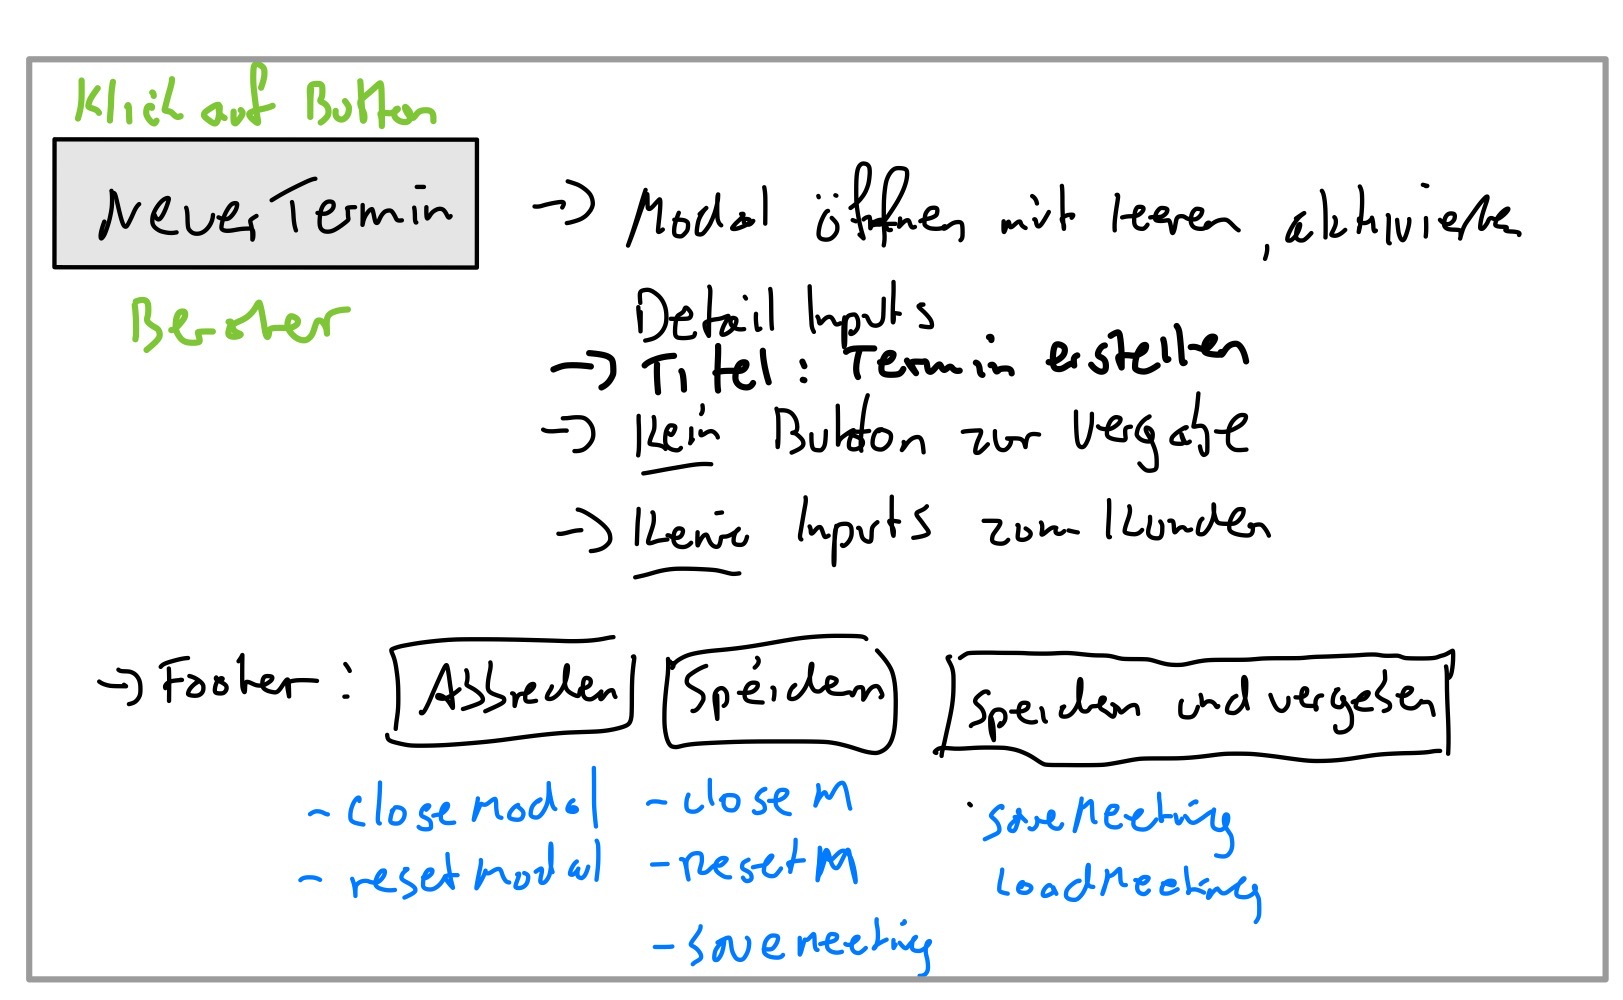
\includegraphics[width=\textwidth]{flow_neuer_termin.jpeg}
\end{figure}

\begin{figure}[H]
    \caption{Sequenzdiagramm, Laden der Detailansicht für einen freien Termin}
    \centering
    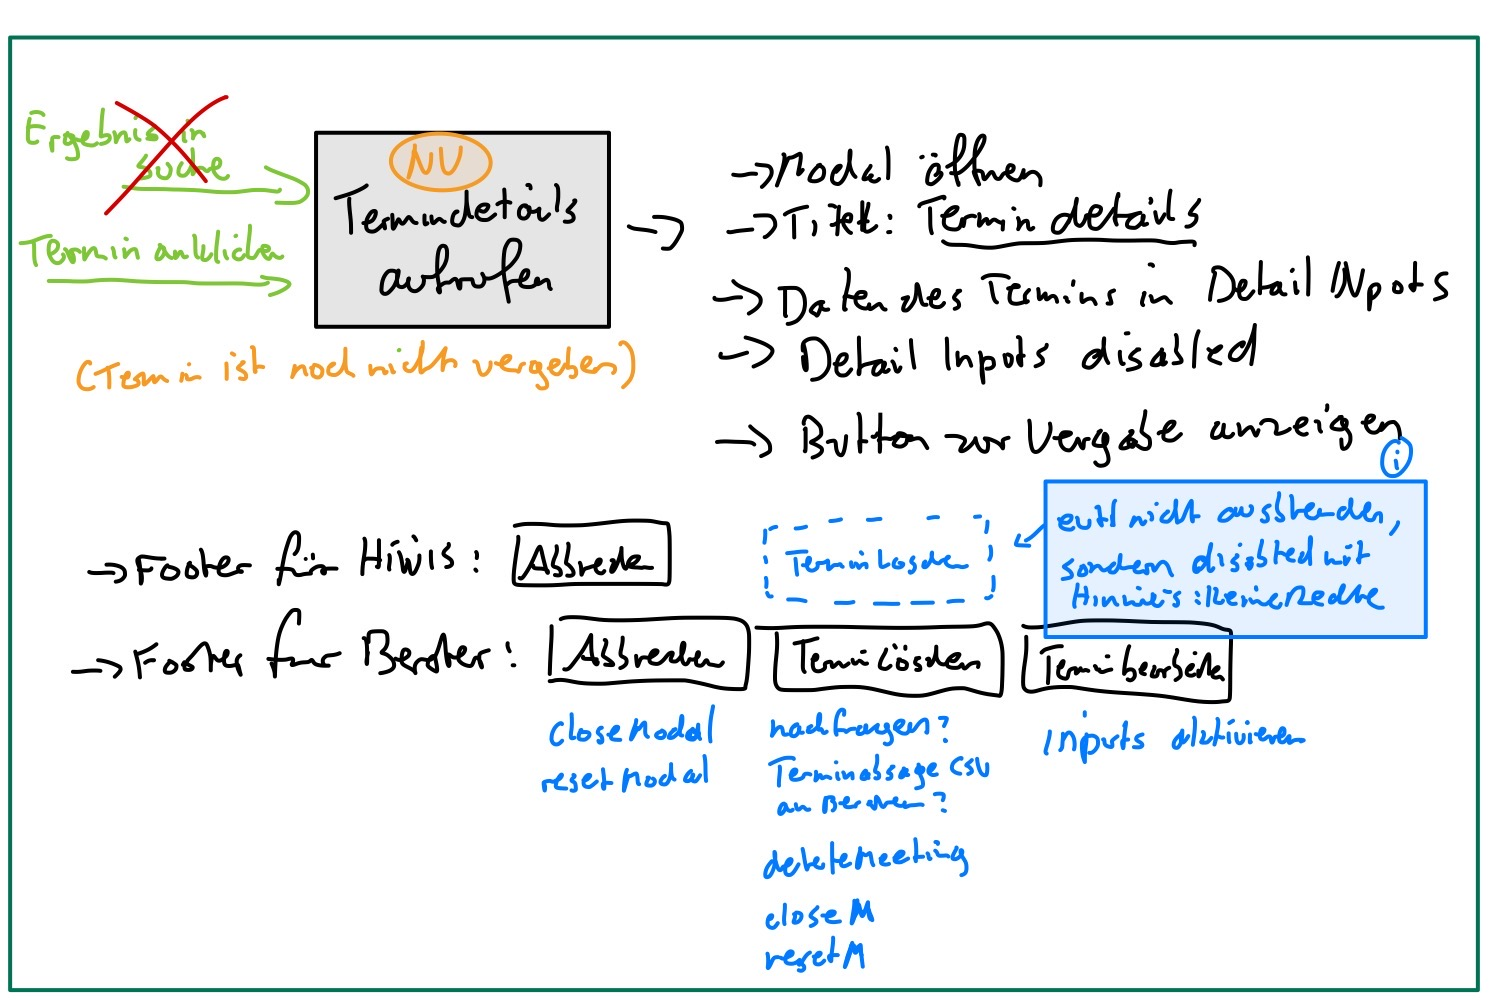
\includegraphics[width=\textwidth]{flow_termin_aufrufen_unvergeben.jpeg}
\end{figure}

\begin{figure}[H]
    \caption{Sequenzdiagramm, Laden der Detailansicht für einen vergebenen Termin}
    \centering
    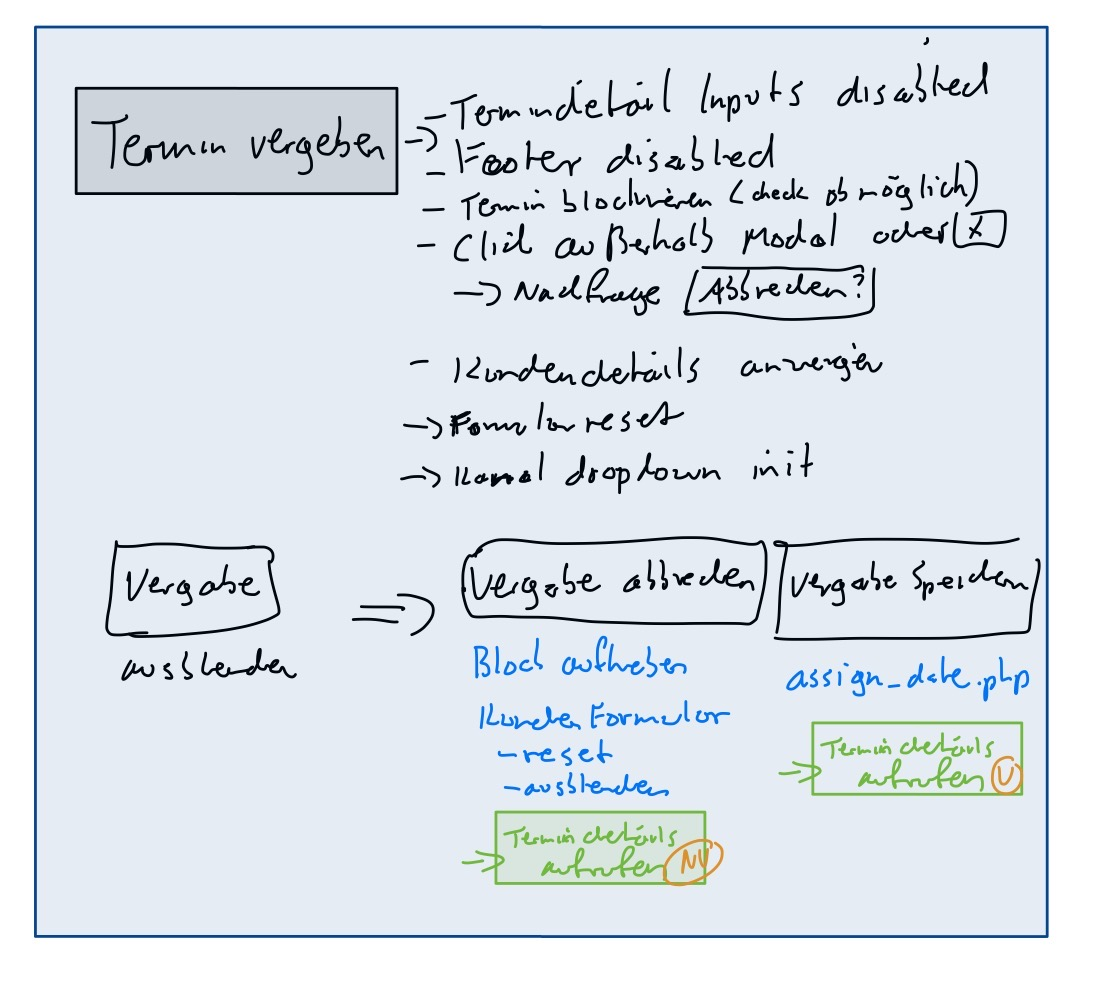
\includegraphics[width=\textwidth]{flow_termin_vergeben.jpeg}
\end{figure}

\begin{figure}[H]
    \caption{Sequenzdiagramm, Vergeben eines Termins und Eintragen der Kundendaten}
    \centering
    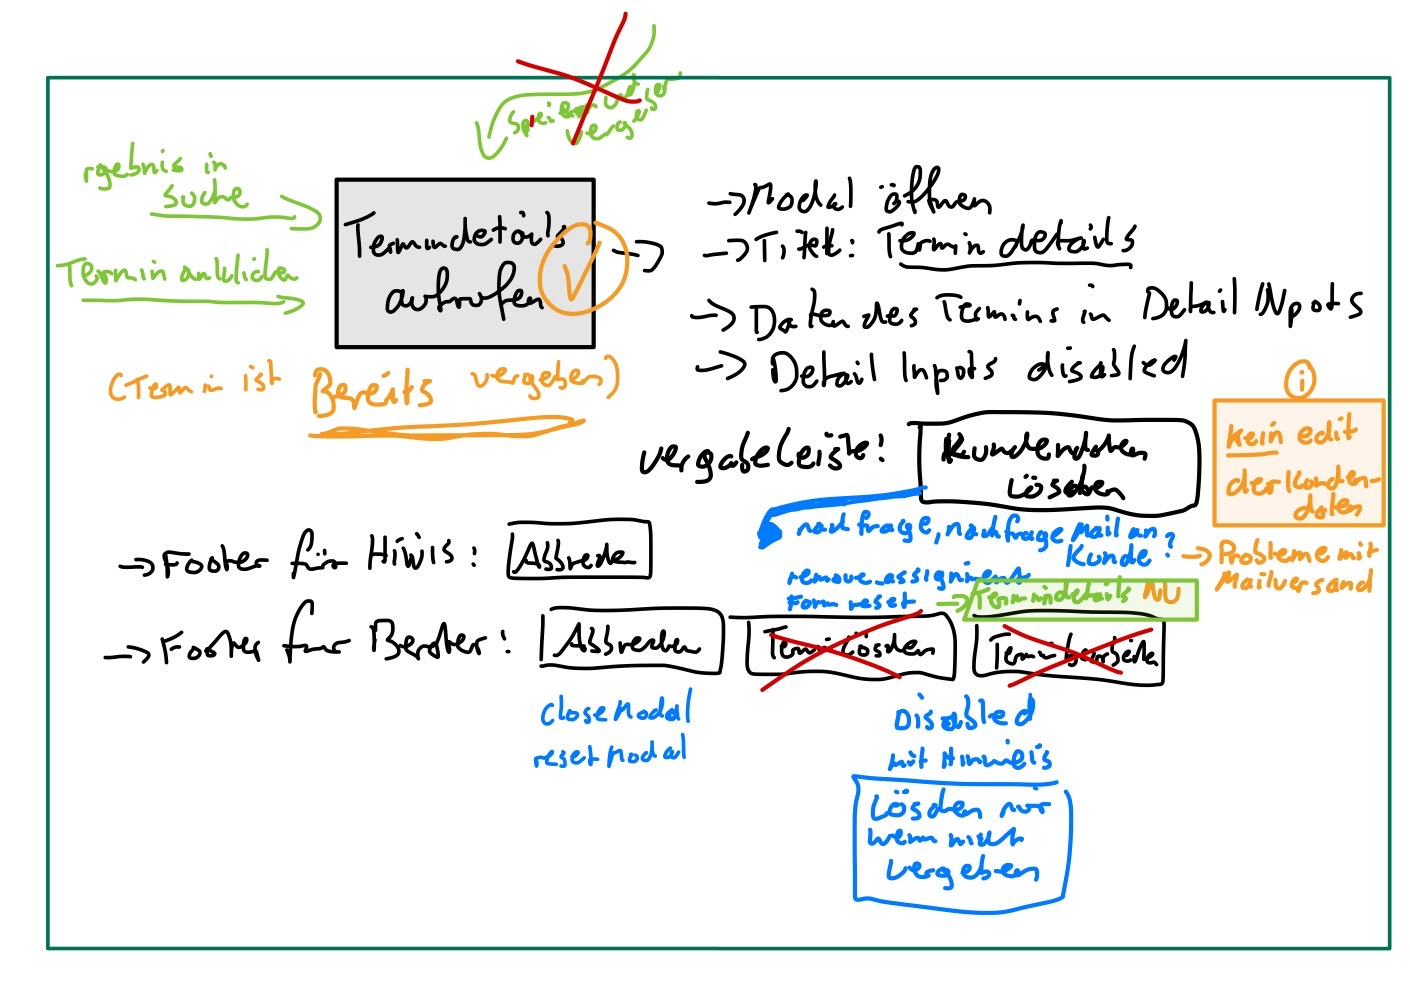
\includegraphics[width=\textwidth]{flow_termin_aufrufen_vergeben.jpeg}
\end{figure}

